\documentclass[11pt,a4paper]{article}

% Basic packages
\usepackage[top=0in,left=0in,right=0in,bottom=0.6in]{geometry}
\usepackage[T1]{fontenc}
\usepackage[utf8]{inputenc}
\usepackage[sfdefault]{FiraSans}
\usepackage{hyperref}
\usepackage{enumitem}
\usepackage{xcolor}
\usepackage{paracol}
\usepackage{graphicx}
\usepackage{tabularx}
\usepackage{tikz}
\usepackage{eso-pic}
\usepackage{changepage}
\usepackage{fontawesome5}

% Styling
\definecolor{sidebar}{HTML}{E4E8ED}
\definecolor{headergray}{HTML}{E4E8ED}
\definecolor{darkbar}{HTML}{3B3B3B}
\definecolor{accent}{HTML}{1F4E79}
\hypersetup{colorlinks=true, urlcolor=accent}
\pagecolor{white}
\pagestyle{empty}
\setlength{\parindent}{0pt}
\setlength{\fboxsep}{0pt}
\setlength{\tabcolsep}{0pt}
\setlength{\columnsep}{0pt}
\setlength{\columnseprule}{0pt}
\columnratio{0.28,0.72}
\setlist[itemize]{leftmargin=1.6em, labelsep=0.5em, itemsep=0.2em, topsep=0.2em}

% Helper commands
\newcommand{\leftsection}[1]{
    \vspace{0.6em}
    {\bfseries #1}\\
    \vspace{0.2em}
    \noindent\hspace*{-0.2cm}\rule{\dimexpr\linewidth-2.0cm\relax}{0.4pt}\\
    % \vspace{0.4em}\par
}

\newcommand{\rightsection}[1]{
    \vspace{0.8em}
    {\large\bfseries #1}\\
    \vspace{0.2em}
    \noindent\hspace*{-0.4cm}\rule{\dimexpr\linewidth+0.4cm\relax}{0.4pt}
    \vspace{0.4em}
}

\newcommand{\entry}[4]{
    \textbf{#1} \hfill {#2}\\
    \textit{#3} \hfill \textit{#4}\\
}

\newlength{\photoht}
\newlength{\photowd}
\newlength{\photorad}
\newlength{\barht}
\newlength{\headerpad}
\newlength{\photopad}  
\newlength{\summarypad}
\newlength{\sidepad}
\newlength{\mainpad}
\newlength{\leftpanelwd}
\setlength{\photoht}{4.5cm}
\setlength{\photowd}{4.5cm}
\setlength{\photorad}{0.5\photowd}
\setlength{\barht}{0.75cm}
\setlength{\headerpad}{0.5cm}
\setlength{\photopad}{-0.1cm}
\setlength{\summarypad}{1.0cm}
\setlength{\sidepad}{0.5cm}
\setlength{\mainpad}{1.0cm}
\setlength{\leftpanelwd}{\dimexpr0.33\paperwidth-1cm\relax}

\newcommand{\photobox}{
    \begin{tikzpicture}
        \clip (0,0) circle (\photorad);
        \node at (0,0) {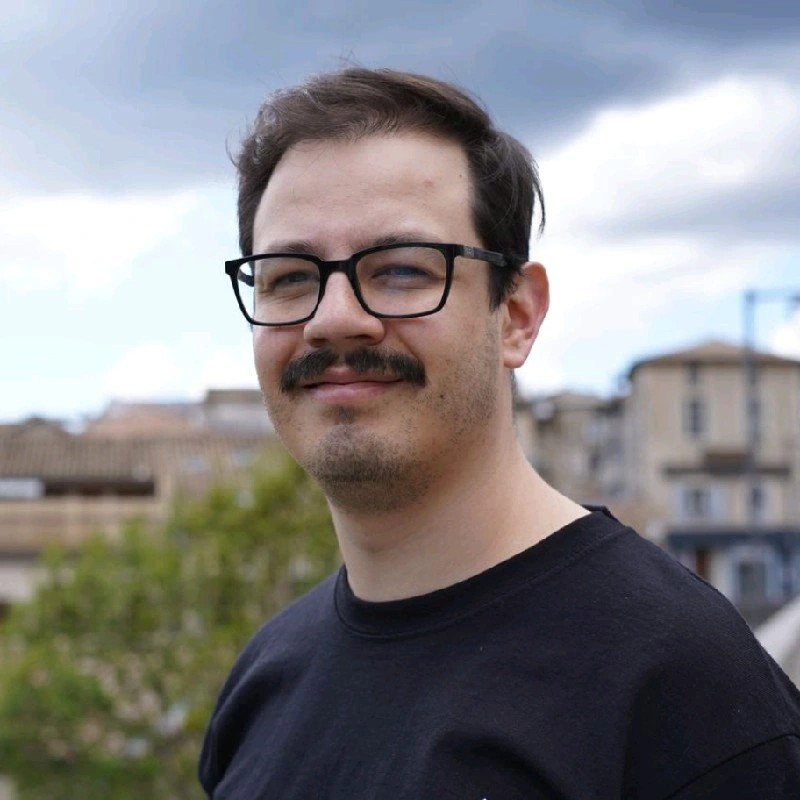
\includegraphics[width=\photowd,height=\photoht]{1745395862968.jpg}};
        \draw[gray!60, line width=0.6pt] (0,0) circle (\photorad);
    \end{tikzpicture}
}

\newcommand{\summarybox}{
    \colorbox{headergray}{
        \begin{minipage}[t][\photoht][t]{\linewidth}
            \vspace*{\headerpad}
            \hspace*{\headerpad}
            \begin{minipage}[t]{\dimexpr\linewidth-2\headerpad-\summarypad\relax}
                {\large\textbf{Battery Systems Engineer and Researcher}}\\
                PhD candidate at TUM with 5+ years of applied research, specializing in data-driven modeling, state estimation, and optimization of grid-scale energy storage. Developed digital twin solutions for second-life battery systems through publicly funded, industry-collaborative research, resulting in 7 peer-reviewed publications (3 as first author).
            \end{minipage}
        \end{minipage}
    }
}

\newcommand{\headerphoto}{
    \colorbox{sidebar}{
        \begin{minipage}[t][\photoht][t]{\linewidth}
            \vspace*{\photopad}
            \hspace*{\headerpad}
            \photobox
        \end{minipage}
    }
}

\newcommand{\namebar}[1]{
    \colorbox{darkbar}{
        \parbox[c][\barht][c]{\paperwidth}{\hspace{\sidepad}\color{white}\bfseries\Large #1}
    }
}% 

\begin{document}

\AddToShipoutPictureBG*{\AtPageLowerLeft{\color{sidebar}\rule{\leftpanelwd}{\paperheight}}}

\noindent
\colorbox{headergray}{%
    \begin{tabularx}{\paperwidth}{@{}p{\leftpanelwd}@{}X@{}}
        \headerphoto &
        \summarybox    \\
    \end{tabularx}%
}%
\noindent
\vspace*{-1pt}
\namebar{MARTIN CORNEJO}

\vspace{0.3em}

\begin{paracol}{2}
    \columncolor{sidebar}
    \color{black}
    \setlength{\leftskip}{\sidepad}
    \setlength{\rightskip}{\sidepad}

    \faMapMarkerAlt\ Munich, Germany\\[0.5cm]
    \faPhone\ +49 173 5714732\\[0.5cm]
    \faEnvelope\ \href{mailto:martincornejo@proton.me}{martincornejo@proton.me}\\[0.4cm]
    \faLinkedinIn\ \href{https://linkedin.com/in/martin-cornejo-v}{martin-cornejo-v}\\[0.4cm]
    \faOrcid\ \href{https://orcid.org/0009-0008-0560-9620}{0009-0008-0560-9620}\\[0.4cm]
    \faGithub\ \href{https://github.com/martincornejo}{github.com/martincornejo}

    \vspace{0.5cm}
    \leftsection{Technical Skills}
    \textbf{Programming:} \\
    Python, Julia, MATLAB\\[0.2cm]

    \textbf{Libraries:} \\
    pyomo, pandapower, \\
    JuMP, ModelingToolkit,\\
    SciML ecosystem\\[0.2cm]

    \textbf{Development:} \\
    SimSES (Python), \\
    RecursiveGPs.jl (Julia)\\[0.2cm]

    \textbf{Tools:} \\
    Git, Docker, Linux, \\GitHub CI

    \vspace{0.5cm}
    \leftsection{Languages}
    Spanish -- Native\\
    English -- C1 \\
    German -- C1 \\
    Italian -- B1 \\
    Armenian -- A2 \\

    % Right column body
    \switchcolumn
    \columncolor{white}
    \color{black}
    \begin{adjustwidth}{\mainpad}{\mainpad}

        \vspace{-0.1cm}
        \rightsection{Experience}
        \entry{Research associate}{03/2021 -- Present}{TUM -- Chair of Electrical Energy Storage Technology}{}
        \vspace{-0.3cm}
        \begin{itemize}
            \item Developed data-driven models and digital twin frameworks for second-life battery storage systems in the publicly funded KI-M-Bat project, in collaboration with Kempten University of Applied Sciences, Fenecon, and STABL Energy.
            \item Team lead (6 members) for Application and System Integration: coordinated research planning and contributed to acquisition of multiple publicly funded projects.
            \item Supervised 37 student works (20 projects, 11 Master's and 6 Bachelor's theses); conducted tutorials for two lectures and one laboratory course.
        \end{itemize}
        \vspace{0.5cm}

        \entry{Working student}{03/2019 -- 11/2020}
        {Siemens Corporate Technology -- Energy System Modelling Group}{}
        \vspace{-0.3cm}
        \begin{itemize}
            \item Data acquisition, preprocessing, and analysis supporting multiple energy system models deployed in industry projects.
            \item Applied machine learning and image recognition techniques in a collaboration with the Siemens AI Lab to detect wind turbines in satellite imagery.
        \end{itemize}
        \vspace{0.5cm}

        % \entry{Research internship}{08/2018 -- 10/2018}
        % {Deutsche Gesellschaft für Internationale Zusammenarbeit (GIZ) - Ecuador}{}
        % \vspace{-0.2cm}
        % \begin{itemize}
        %     \item Research on regulatory and policy framework for electromobility in Ecuador, under the ``Sustainable Intermediate Cities'' program.
        %     \item Assisted in organizing the ``1st International Forum on Electromobility'' (Cuenca, Ecuador, September 2018).
        % \end{itemize}

        \vspace{0.1cm}
        \rightsection{Education}
        \entry{Doctor of Engineering (in progress)}{03/2021 -- Present}
        {TUM -- Chair of Electrical Energy Storage Technology}{}
        Thesis: Field-Data-Driven Digital Twins for Modeling and Optimization of Second-Life Battery Storage Systems.
        \\[0.2cm]

        \entry{Master of Science Electrical Engineering \\and Information Technology}{04/2018 -- 01/2021}
        {Technical University of Munich}{}
        Grade: 1,6 (Passed with Merit) \\
        % Specialization: Power Engineering\\
        Master's Thesis: A decentralized optimal power flow method for real-time \\applications in power distribution systems.\\[0.2cm]

        \entry{Bachelor of Science Electrical Engineering \\and Information Technology}{10/2014 -- 03/2018}
        {Technical University of Munich}{}
        Grade: 2,3 (Passed with Merit) \\
        Bachelor's Thesis: Cost analysis of solar air conditioning systems.

        % \rightsection{Certifications}
        % Basis Certificate in Project Management (GMP)

        % \rightsection{References}
        % References available on request.

    \end{adjustwidth}

\end{paracol}

% \newpage
% \AddToShipoutPictureBG*{\AtPageLowerLeft{\color{sidebar}\rule{\leftpanelwd}{\paperheight}}}
% \vspace*{0.6cm}
% \begin{adjustwidth}{\dimexpr\leftpanelwd+\mainpad\relax}{\mainpad}

%     \rightsection{Selected Publications}
%     \textit{First author}
%     \begin{itemize}
%         \item \textbf{Cornejo, M.} et al. (2025). Data-driven model enhancement of late-life lithium-ion batteries. \textit{Future Batteries}, 6, 100060.
%         \item \textbf{Cornejo, M.} et al. (2025). Evaluating the Impact of Model Accuracy for Optimizing Battery Energy Storage Systems. \textit{IEEE ISGT Europe 2025}.
%         \item \textbf{Cornejo, M.} et al. (2022). PHIL implementation of a decentralized online OPF for active distribution grids. \textit{IEEE PESGM 2022}.
%     \end{itemize}
%     \vspace{0.3cm}
%     \textit{Co-author}
%     \begin{itemize}
%         \item Collath, N., \textbf{Cornejo, M.} et al. (2023). Increasing the lifetime profitability of battery energy storage systems through aging aware operation. \textit{Applied Energy}, 348, 121531.
%     \end{itemize}
% \end{adjustwidth}

\end{document}
